%%
%% ****** Generated 24.03.23 by LJM TeX-constructor******
%%
\documentclass{article}

\usepackage{amssymb}
\usepackage{amsfonts}
\usepackage[tbtags]{amsmath}
\usepackage{amscd}
\usepackage{amsthm}			% Продвинутая математика
\usepackage{mathtext}
\usepackage{cmap}
\usepackage[T2A]{fontenc}
\usepackage[utf8]{inputenc}			% cp1251
\usepackage[english, russian]{babel}
%\usepackage{literat}
\usepackage{pifont}
\usepackage{bm}
\usepackage{array}			% Ширина столбиков в массиве
\usepackage{dcolumn}
\usepackage{hhline}
\usepackage{multirow}
\usepackage{graphicx}
\usepackage{rotating}
\usepackage{calc}
\usepackage{tabularx}
\usepackage{afterpage}
\usepackage{ifthen}
\usepackage{caption2}
\usepackage{substr}
\usepackage[mathscr]{eucal}  %% My addition
\usepackage{mathrsfs}        %% My addition
\usepackage{hypbmsec}        %% My addition
\usepackage{latexsym}        %% My addition
\usepackage{xypic}           %% My addition
\RequirePackage{soul}
\RequirePackage{verbatim}    %% My addition
\RequirePackage{chapterbib}
\RequirePackage{enumerate}


\usepackage[shortcuts]{extdash}
\usepackage{ragged2e}
\usepackage{etoolbox}
\usepackage{lipsum}

%\usepackage{flafter}
\usepackage[section,above,below]{placeins}

\usepackage{indentfirst}
\usepackage[a4paper, top=20mm, left=30mm, right=20mm, bottom=25mm]{geometry}


\setcounter{page}{1}

\begin{document}
\title{Восстановление полей гидропроводности и упругоемкости нефтяных пластов на основе решения обратной задачи с использованием сети радиальных базисных функций} % for running heads
\author{Косяков В.П., Легостаев Д.Ю.} % for running heads

%\noaffiliation % If the author does not specify a place of work.

%\firstcollaboration{(Submitted by ) } % Add if you know submitter.
%\lastcollaboration{ }


\begin{abstract} % You shouldn't use formulas and citations in the abstract.
В нефтяной отрасли наблюдается заметная тенденция к использованию прокси-моделей различных уровней сложности для выполнения оперативных прогнозных расчетов, в частности, к методам машинного обучения, которые активно развиваются в контексте цифровизации и интеллектуализации производственных процессов. В этой статье на примере элемента разработки модели синтетического нефтяного пласта мы представляем подход к совместному использованию физически значимой модели потока жидкости и методов машинного обучения для решения задач адаптации и прогнозирования. Особенностью синтетической модели является наличие выраженных зональных неоднородностей полей проницаемости и упругоёмкости. В рамках предложенного подхода была использована упрощенная фильтрационная модель, которая была настроена на исторические значения параметров разработки за счёт восстановления полей фильтрационных параметров коллектора. Восстановление полей выполнялось при использовании сети радиальных базисных функций. На основе восстановленных полей фильтрационных параметров были рассчитаны коэффициенты связи между скважинами, которые качественно и количественно соответствуют истинным значениям. Прогнозные характеристики предлагаемого подхода оценивались при помощи разбиения исторического набора данных на обучающие и тестовые интервалы.
\end{abstract}

\textbf{Keywords}:flow through porous medium, reservoir mathematical simulation, inverse problem, adjoint problem, machine learning, radial basis functions% Include keywords separeted by comma.

\maketitle

% Text of article starts here.
\section{INTRODUCTION}

В настоящее время в нефтедобывающей отрасли, наряду с использованием традиционных гидродинамических моделей, широко применяется использование упрощённых прокси-моделей. Использование упрощённых моделей позволяет сократить вычислительные затраты, а также снизить требования к качеству и полноте исходных данных. Развитие и применение прокси-моделирования для обратных и оптимизационных задач является актуальным, так как они являются самыми ресурсоёмкими задачами. Помимо физически содержательных моделей (материальный баланс \cite{mus1}, супер элементы, CRM \cite{bek}, линии тока \cite{pot}, многофазные фильтрационные модели \cite{ele}, \cite{kos} и т.д.), развиваются подходы, основанные на применении методов машинного обучения \cite{tem}, \cite{uma}. Например, рекуррентные нейронные сети получили применение в области прогнозирования временных рядов и, в частности, режимов работы скважин. Однако, применение подходов, основанных только на методах машинного обучения, в качестве прогнозирующих моделей не может гарантировать получения верного с точки зрения физики процесса результата. Совместное использование физически содержательной модели и методов машинного обучения позволяет избегать проблем подобного рода \cite{kos2}.

На рисунке \ref{fig:schime1} представлена общая схема используемого подхода. Алгоритм работы заключается в том, что методы машинного обучения объединяются с физически содержательной фильтрационной моделью, которая используется в качестве одного из слоёв полученной “гибридной” нейронной сети. При данном подходе на вход блока машинного обучения подается одна часть данных «input ML», рассчитываются значения «output ML», которые вместе со второй частью данных «input Flow» выступают в качестве входа для расчета «Flow». Для настройки параметров модели «ML» используются результаты решения сопряженной задачи («Flow derivative»), которые позволяют рассчитать градиент для фильтрационной части. Расчёт градиента для элементов МО выполняется с помощью стандартной процедуры обратного распространения ошибки. Для ФМ расчёт градиента является отдельной трудоёмкой задачей, вычислительная сложность которой, как правило, сопоставима или превосходит сложность прямого расчёт ФМ. Расчёт градиента для ФМ вынесен в отдельный блок решения сопряжённой задачи.

\begin{figure}
	\centering
	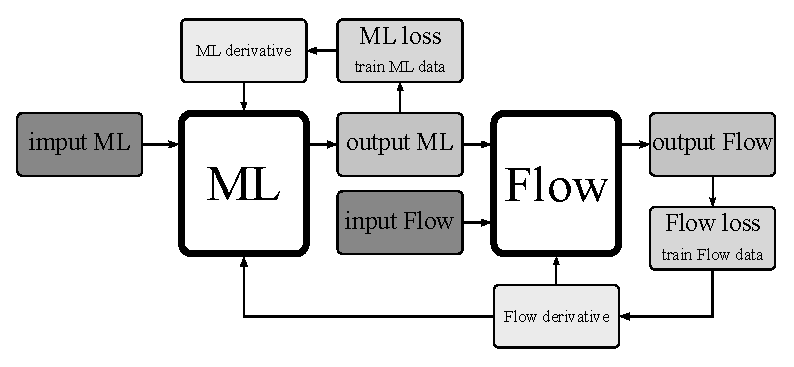
\includegraphics[width=0.7\linewidth]{images/fig1.eps}
	\caption{Схема алгоритма совместного использования машинного обучения и однофазной фильтрационной модели.}
	\label{fig:schime1}
\end{figure}


Целью настоящей работы является развитие инструментов прокси-моделирования на основе теории фильтрации и элементов машинного обучения. Задача восстановления фильтрационно-ёмкостных параметров пластовой системы в межскважинном пространстве при помощи сети радиально-базисных функций была решена путем адаптации фильтрационной модели на известные значения пластового давления при заданных расходах жидкости на скважинах. Для контроля прогностических свойств моделей проведено разбиение моделируемого периода разработки на обучающий и тестовый интервалы.

\section{Mathematical Model}

\subsection{Single-phase flow model}
Для решения этой задачи в качестве модели фильтрации была использована двумерная математическая модель однофазного течения
слабосжимаемой жидкости:

\begin{equation} \label{fil}
	\triangledown \cdot \left[\frac{k}{\mu}\triangledown P \right] = \beta^* \frac{\partial P}{\partial t} + \delta(x_1,x_2),
\end{equation}

\begin{equation} \label{bc}
	\delta(x_1,x_2)  = \left\{\begin{array}{crl}
		0, \;\mbox{if}\;(x_1,x_2) \notin\ \Gamma_{in}\cup\Gamma_{out},\\
		q_{i}, \;\mbox{if}\;(x_1,x_2) \in \Gamma_{in},\\
		q_{a}, \;\mbox{if}\;(x_1,x_2) \in \Gamma_{out},
	\end{array}\right. 
\end{equation}
Замыкающие соотношения:
\begin{equation} \label{kr}
P = P_0\mbox{,\quad \mbox{if} $t=0$},
\end{equation}
где $k$ --- проницаемость, $P$ --- пластовое давление, $\beta^*$ --- эффективная сжимаемость, $q_i$ is fluid flow rate in $i$th well, $\Gamma_{in}$ --- множество источников/стоков (скважин), $\Gamma_{out}$ --- внешняя граница, $P_0$ --- начальное пластовое давление при $t=0$, $q_{a}$ --- расход жидкости через внешнюю  границу, который может быть представлен как:
\begin{equation*} \label{qaq}
	q_a = T_a(P_{a} - P|_{\Gamma_{out}}),
\end{equation*}
где $P_a$ --- давление в аквифере ($P_a = P_0$), $T_a$ --- 
проводимость границы водоносного горизонта (включает коэффициент продуктивности водоносного горизонта). Целью решения обратной задачи является нахождение проницаемости $k = k(x_1,x_2)$ и эффективной сжимаемость $\beta^* = \beta^*(x_1,x_2)$ при котором расчётные значения пластового давления и расхода будут удовлетворительно совпадать с исходными значениями соответствующих параметров.

\subsection{RBF}

Получение значений $k(x_1,x_2)$ и $\beta^*(x_1,x_2)$ возможно различными способами, например интерполяция и экстраполяция измеренных значений вблизи скважин в область межскваженного пространства. В настоящей работе предлагается получение искомых значений при использовании модели машинного обучения. В качестве модели машинного обучения была выбрана двухслойная нейронная сеть, состоящая из слоя радиально-базисных функций (РБФ) и полносвязного слоя. Слой РБФ определяет влияние каждого базиса на выбранную точку пространства.

При решении обратной задачи удобнее от проницаемости $k$ перейти к общей подвижности $\lambda$, при помощи этого параметра можно комплексно учесть множество фильтрационных параметров влияющих на структуру фильтрационных потоков (вязкость, относительные фазовые проницаемости и т.д.). От эффективной сжимаемости $\beta^*$ удобнее перейти к параметру упругоёмкости $\beta$, который позволяет комплексно оценить упруго-ёмкостные характеристики.
Поля общей подвижности $\lambda$ и эффективной сжимаемости $\beta$ рассматриваются в виде функциональной зависимости $\lambda(\mathbf{x})$ и $\beta(\mathbf{x})$, где  $\mathbf{x} = (x_1, x_2)$ --- вектор пространственных координат. В качестве зависимости использована сеть радиально базисных функций.

\begin{eqnarray}\label{rbf}
	f_i(\mathbf{x}) = exp \left(\frac{-\lVert \mathbf{x} - \mathbf{c_f}_i \rVert^2}{\epsilon_{fi}^2}\right), \quad
	g_i(\mathbf{x}) = exp \left(\frac{-\lVert \mathbf{x} - \mathbf{c_g}_i \rVert^2}{\epsilon_{gi}^2}\right),
\end{eqnarray}

\begin{eqnarray}
	\lambda(\mathbf{x}) = w_{fi}f_i + b_h, \quad
	\beta(\mathbf{x}) = w_{gi}g_i + b_g,
\end{eqnarray}
где $\mathbf{x}$ – координаты расчетных узлов,  $\mathbf{c_f}_i$ и $\mathbf{c_g}_i$– положение базисов, $\epsilon_{fi}$ и $\epsilon_{gi}$– ширина базисов, $w_{fi}$ и $w_{gi}$ – веса базисов, $b_f$ и $b_g$ – свободный член. Параметры сети радиально базисных функций $\mathbf{c}_i$, $\epsilon_i$, $w_i$, $b$  настраиваются в процессе адаптации однофазной фильтрационной модели.

\subsection{INVERSE PROBLEM}

Обратная задача решается в оптимизационной постановке, которая заключается в минимизации целевой функции $J$.
Целевая функция может быть записана в виде суммы слагаемых, каждое из которых является произведением функции, характеризующей отклонение вычисленных значений от контрольных, и весового коэффициента для соответствующего типа переменной. В качестве меры отклонения была выбрана среднеквадратичная ошибка (MSE).
\begin{equation} \label{mse}
	J=\frac{w_p}{N_p}\sum_{i=1}^{N_p}{\left(p_c^i-p_f^i\right)^2}+
	\frac{w_{\lambda}}{N_\lambda}\sum_{i=1}^{N_\lambda}{\left(\Delta\lambda^i  \right)^2}+
	\frac{w_{\beta}}{N_\beta}\sum_{i=1}^{N_\beta}{\left(\Delta\beta^i  \right)^2},
\end{equation}
\begin{equation} \label{mse1}
	\Delta\lambda^i  = \left\{\begin{array}{crl}
		\lambda^i_c - \lambda^i_r, \quad \;\mbox{if}\; \lambda^i_c \ge \lambda^i_r\\
		0,\quad \;\mbox{if}\; \lambda^i_l < \lambda^i_c < \lambda^i_r\\
		\lambda^i_c - \lambda^i_l, \quad \;\mbox{if}\;\lambda^i_c \le \lambda^i_l
	\end{array}\right.,
	\quad
	\Delta\beta^i  = \left\{\begin{array}{crl}
		\beta^i_c - \beta^i_r, \quad \;\mbox{if}\; \beta^i \ge \beta^i_r\\
		0,\quad \;\mbox{if}\; \beta^i_l < \beta^i_c < \beta^i_r\\
		\beta^i_c - \beta^i_l, \quad \;\mbox{if}\;\beta^i_c \le \beta^i_l,
	\end{array}\right.
\end{equation}	
где $p_c^i$ --- расчетное значение пластового давления, $p_f^i$
- фактическое значение, $i$ --- номер измерения, $N_p$ ---
количество измерений пластового давления,$N_\lambda$ ---
количество известных значений подвижности и $N_\beta$ --- это число известных значений эффективной сжимаемости. $\lambda$ --- истинное значение подвижности на скважине, $\lambda_c$ --- расчетное значение подвижности,  $\lambda_l$ и $\lambda_r$ --- левое и правое ограничение на значение общей подвижности подвижность, $\beta$ --- расчетное значение упругоёмкости,  $\beta_l$ и $\beta_r$ --- левое и правое ограничение на значение эффективной упругоёмкости.  
Индекс $f$ означает фактические значения (fact), а $c$ --- рассчитанные (calculated), $w_p$, $w_\lambda$ и $w_\beta$ --- весовые коэффициенты, учитывающие степень влияния различных параметров (размерность, качество данных и т.д.). Аргументами целевой функции, ответственными за давление, являются фактические (измеренные) и расчетные значения пластового давления в месте расположения скважины в заданные моменты времени.

Второе и третье слагаемое целевой функции {\ref{mse}} отвечает за настройку поля подвижности и упругоёмкости на известные значения фильтрационно-ёмкостных свойства пласта. Причем рассчитанные значения подвижность и упругоёмкости могут изменяться в диапазоне значений от $\lambda_l$ до $\lambda_r$ и $\beta_l$ до $\beta_r$, не приводя к росту целевой функции. Наличие допустимого интервала связано с изменением во времени фазового состава на скважинах, влияющего на подвижность и упругоёмкость в прискважинной зоне. 

При использовании градиентного метода оптимизации, необходимо найти компоненты градиента
целевой функции, которые можно записать в следующем виде:

\begin{equation}\label{grad}
	\frac{\partial J}{\partial u_k} = 
	2w_p\frac{1}{N}\sum_{i=1}^N	({p_c^i-p_f^i}) \frac{\partial p_c^i}{\partial u_k}+
	2w_{\lambda}\frac{1}{N_\lambda}\sum_{i=1}^{N_\lambda}{\Delta\lambda^i}\frac{\partial
		\lambda_{c}^i}{\partial u_k}+
	2w_{\beta}\frac{1}{N_\beta}\sum_{i=1}^{N_\beta}{\Delta\beta^i}\frac{\partial
			\beta_{c}^i}{\partial u_k}.
\end{equation}
Для решения оптимизационной задачи необходимо, чтобы каждая компонента градиента целевой функции стремилась к 0, что можно записать следующим образом:
\begin{equation} \label{rp}
	\frac{\partial J}{\partial u_k} \rightarrow 0.
\end{equation}

Для решения обратной задачи градиентным методом необходим расчёт компонент градиента целевой функции по настраиваемым параметрам. В качестве настраиваемых параметров выступают параметры RBF \ref{rbf}. Компоненты градиента целевой функции:
\begin{equation*}
		\frac{\partial J}{\partial w},\quad \frac{\partial J}{\partial \epsilon},\quad \frac{\partial J}{\partial b}, \quad \frac{\partial J}{\partial \mathbf{c}}.
\end{equation*}

В целевую функцию \ref{mse} могут быть добавляются дополнительные слагаемые, которые являются штрафными функциями, позволяющими регуляризировать получаемые решения. Были добавлено слагаемое, позволяющее контролировать положение базисов функций \ref{rbf} относительно друг друга и расчётной области. Целевая функция получала штраф при взаимном близком расположении базисов или выходи их за пределы расчётной области.

\begin{equation*} \label{pnl}
	J_{pnl}=\frac{2w_{dist}}{N_\textbf{x}*(N_\textbf{x}-1)}\sum_{i=1}^{N_\textbf{x}}{\sum_{j=i+1 }^{N_\textbf{x}}{\left(f_{relu}\left(r_{min} - r_{i,j}\right)\right)^2}} + 
	\frac{w_{bnd}}{N_\textbf{x}}\sum_{i=1}^{N_\textbf{x}}{\left(f_{relu}\left(r_{i,c} - \frac{L}{2}\right)\right)^2},
\end{equation*}
где $w_{dist}$ и $w_{dist}$ --- весовые коэффициенты для штрафных функций по расстоянию между базисами и положением относительно границ расчётной области, $N_\textbf{x}$ --- количество базисов, $r_{i,j}$ --- расстояние между i-тым и j-тым базисом,  $r_{min}$ - минимально допустимое расстояние между базисами,  $r_{i,c}$ --- расстояние от i-того базиса до центра расчётной области, $f_{relu}$ --- функция активации (rectified linear unit).

Градиенты вычисляются стандартным для области машинного обучения методом обратного распространения ошибки, который в данном случае предполагает решение сопряженной задач для фильтрационной модели \cite{kos3}, \cite{far}. 
В результате решения сопряженной задачи для фильтрационной модели находятся производные целевой функции по физически содержательным параметрам (подвижность и упругоёмкость) $\frac{\partial J}{\partial \lambda}$ и $\frac{\partial J}{\partial \beta}$. Далее полученные значения передаются модели машинного обучения. В качестве инструмента для реализации представленного подхода была использована библиотека для машинного обучения Flux \cite{inn} языка программирования Julia.

Решение обратной задачи (\ref{rp}) находится численно
итерационным методом. На каждой итерации прямая задача
(\ref{fil})--(\ref{bc}) решается численно. Производные
целевой функции вычисляются в соответствии с настраиваемыми
параметрами модели. Численное решение было найдено
методом контрольного объема для двумерной прямоугольной
разностной сетки с использованием IMPES метода \cite{azi}.

Целевая функция, используемая для решения обратной задачи ({\ref{mse}}), не всегда удобна для субъективной оценки точности модели. Оценка точности сопоставления истории производилась с использованием средней абсолютной процентной ошибки (MAPE). Этот показатель позволяет оценить точность воспроизведения моделью фактического пластового давления, величины подвижности и упругоёмкости вблизи скважин.


\section{RESULTS}

Тестирование предлагаемого подхода выполнено на синтетической модели разработки нефтяного пласта (\ref{fig:schime}) размером 1000х1000 метров с 9 скважинами: 5 добывающими (P1-P5) и 4 нагнетательными (I1-I4), с высокопроводящими включениями $k_1 = 200 мкм^2$ и $k_2 = 100 мкм^2$, проницаемость в основной части расчетной области $k = 20 мкм^2$. Скважины I3, I4, и P5 расположены в зоне повышенной эффективной сжимаемости увеличенной в 2 раза относительно остальной области. 

\begin{figure}
	\centering
	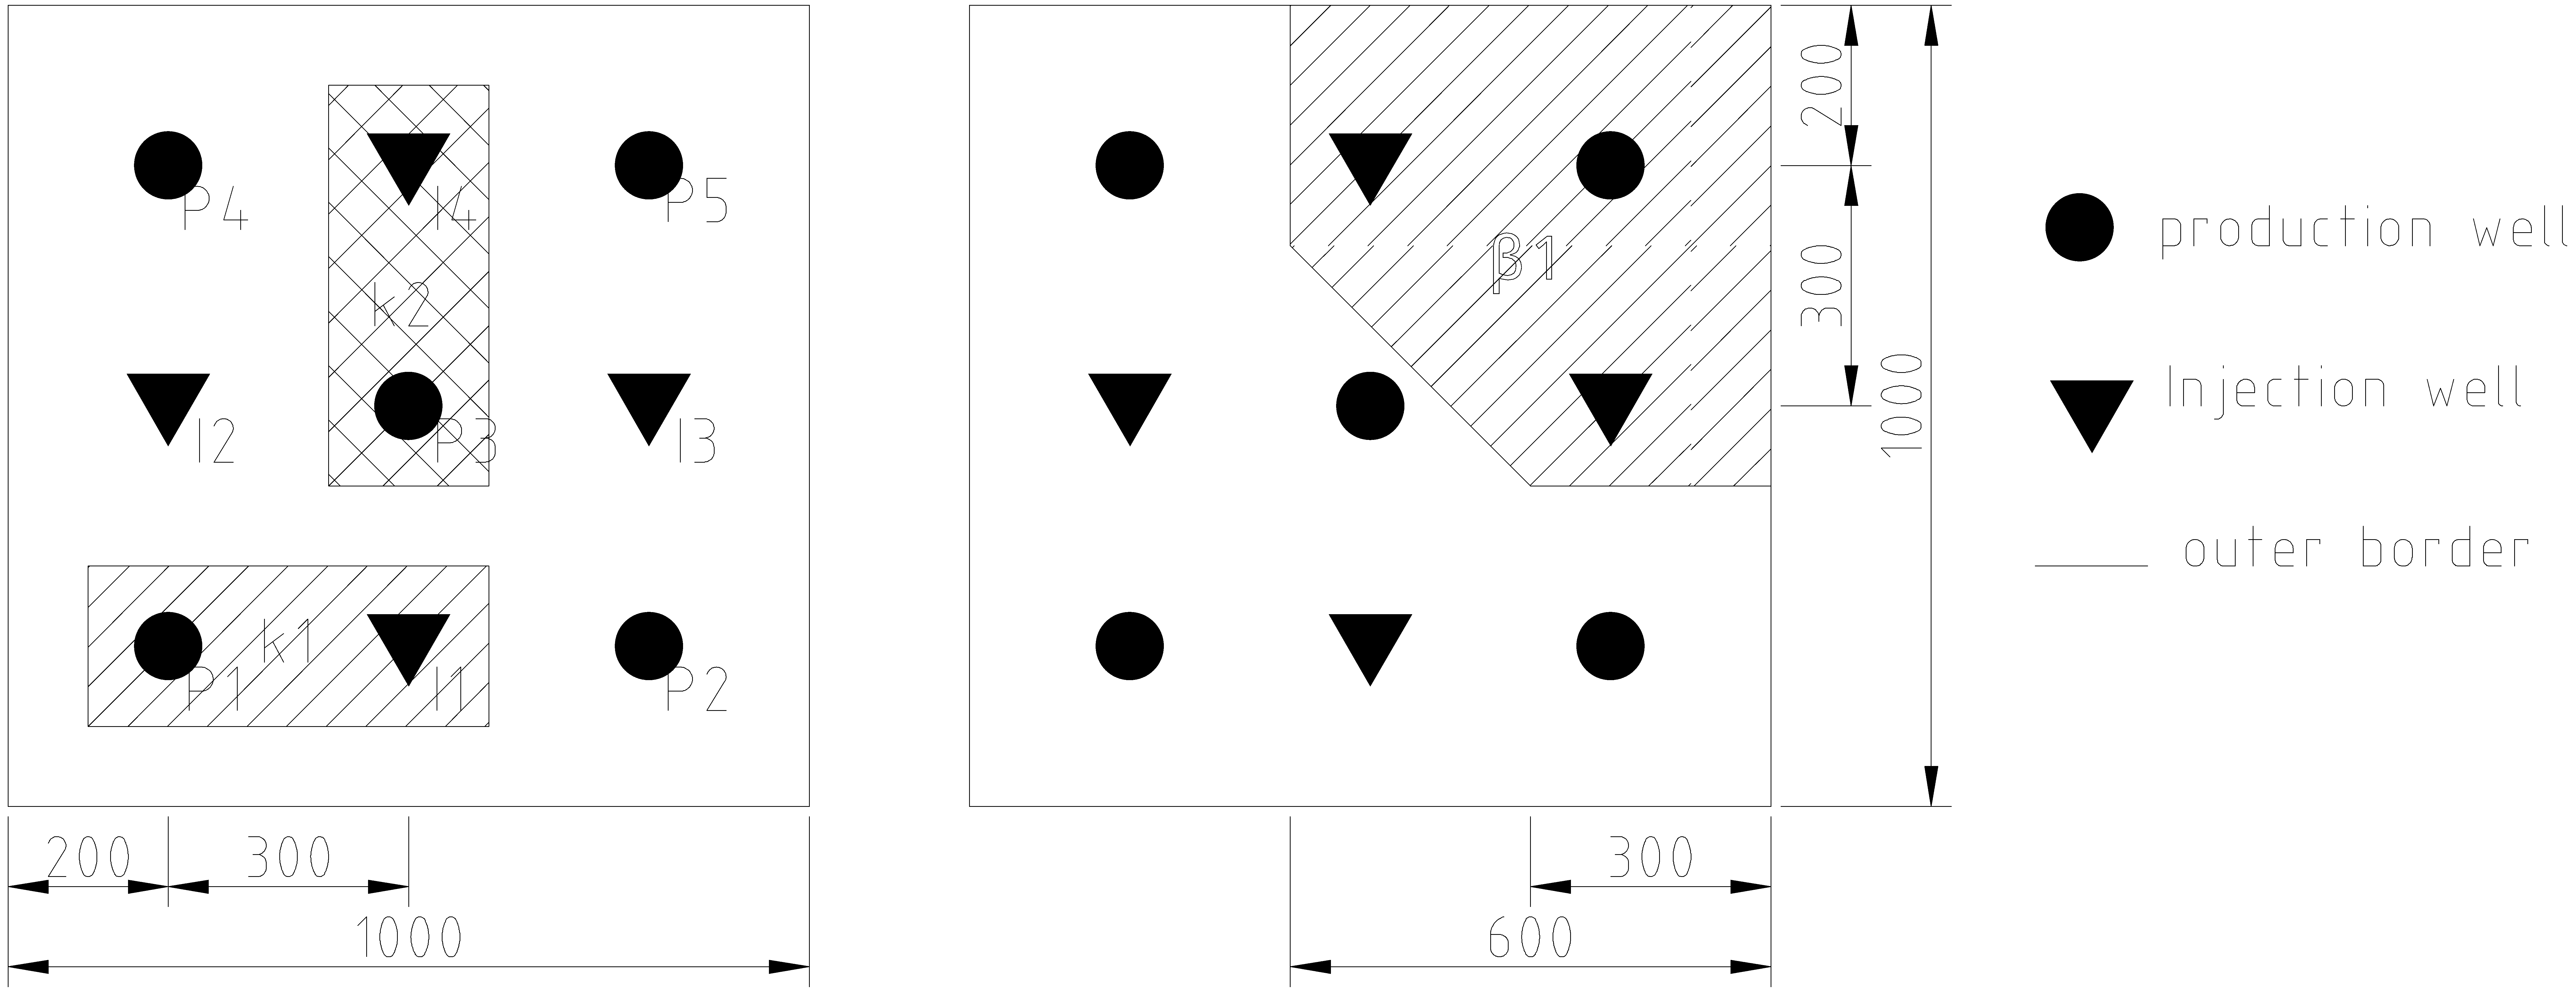
\includegraphics[width=0.7\linewidth]{images/fig2.eps}
	\caption{Schematic representation of the computational domain}
	\label{fig:schime}
\end{figure}

В качестве источника исходных данных была использована синтетическая гидродинамическая модель. Набор данных получен путем прямого численного моделирования двухфазной фильтрации. Полученные данные были использованы для решения задачи адаптации и прогнозирования.
При решении обратной задачи в качестве режимов работы использованы дебиты добывающих скважин и приемистости нагнетательных скважин, полученные из прямого численного моделирования. Пористость, толщина пласта, начальные и граничные условия соответствовали прямой задаче. Обратная задача решается в оптимизационной постановке, в которой минимизируется целевая функция {\ref{mse}}. В качестве фактических замеров пластового давления использовалось ограниченное количество давлений, полученные из решения прямой задачи. Случайным образом выбраны 10\% от общего количества значений пластового давления, которые выступали в качестве истинных значений.

Период моделирования составлял 10 лет, на протяжении которых скважины работали с заданными режимами. Расчетный шаг составлял 1 месяц. Зависимости приемистости нагнетательных скважин от времени, приведенные на рис. \ref{fig:inj_rate}, получены путем случайной генерации и имеют кусочно-постоянный вид. Так же с заданной периодичностью происходит отключение нагнетательных скважин, период простоя составлял от 2 до 4 месяцев. На добывающих скважинах заданы изменяющиеся по гармоническому закону забойные давления, которые приведены на рис. \ref{fig:prod_rate}.

Полученный набор данных был использован для решения обратной задачи. При этом для оценки прогностических свойств модели данные были разделены на обучающую и тестовую выборки. Первые 7 лет истории разработки отнесены к обучающей выборке и использованы для адаптации модели. Период 7-10 лет включен в тестовую выборку для которой проведены прогнозные расчеты. 

\begin{figure}
	\center{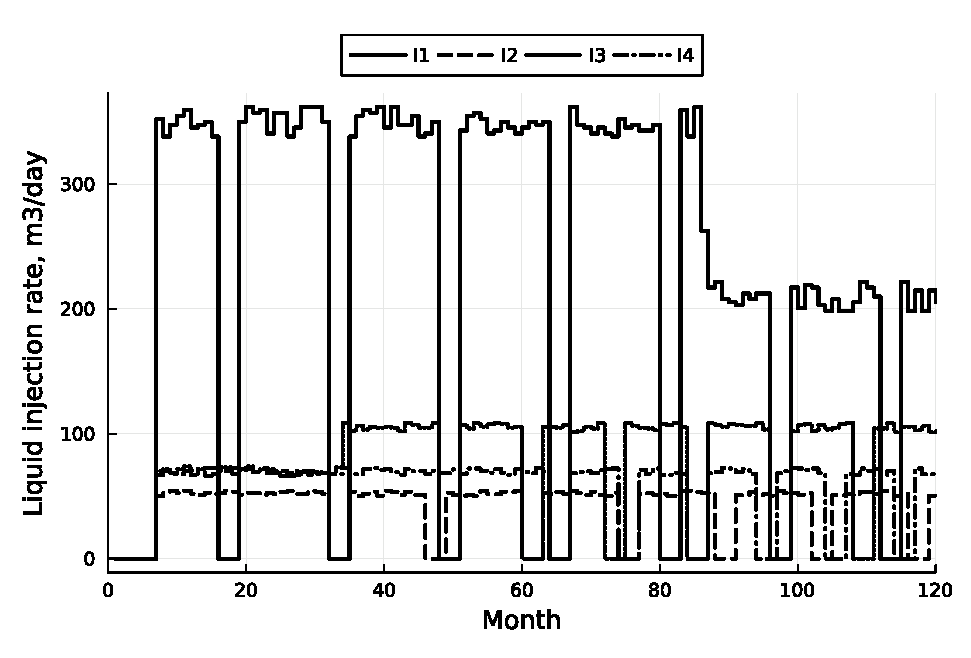
\includegraphics[height=0.40\linewidth]{images/fig3.eps}}
	\caption{Расход жидкости на нагнетательных скважинах I1-I4}
	\label{fig:inj_rate}
\end{figure}

\begin{figure}
	\center{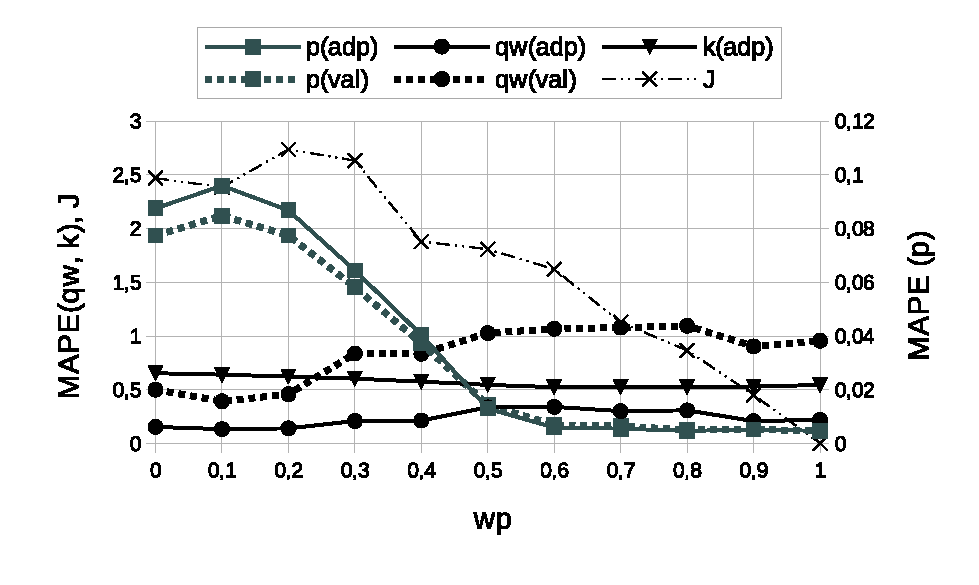
\includegraphics[height=0.40\linewidth]{images/fig4.eps}}
	\caption{Расход жидкости на добывающих скважинах P1-P5}
	\label{fig:prod_rate}
\end{figure}


 Начальное пластовое давление составляло 20 МПа. На границах элемента разработки задано Постоянное пластовое давление $Pa = 20 МПа$. Параметры горной породы и насыщающих ее флюидов, принятые для расчета, имели следующие значения: пористость 0.2, значения абсолютной проницаемости представлены в виде карты на рис. 1, эффективная вязкость 1 мПа*c, толщина пласта принята равной 4 м, эффективная сжимаемость $10^{-4} МПа^{-1}$.

Решение оптимизационной задачи осуществляется встроенными в пакет Flux оптимизационными алгоритмами (Descent и ADAM). В результате решения были получены карты подвижности \ref{fig:mob}a и карты эффективной сжимаемости \ref{fig:comp}b. Несмотря на отличия, видно, что поля качественно повторяют исходные (\ref{fig:schime}).

Восстановленные карты проницаемости и упругоёмкости представлены на рисунках \ref{fig:mob}a и \ref{fig:comp}b. Из рисунков видно, что несмотря на визуальное различие алгоритму удалось качественно воспроизвести основные особенности исходных полей. 

\begin{figure}
	\begin{minipage}[h]{0.48\linewidth}
		\centering
		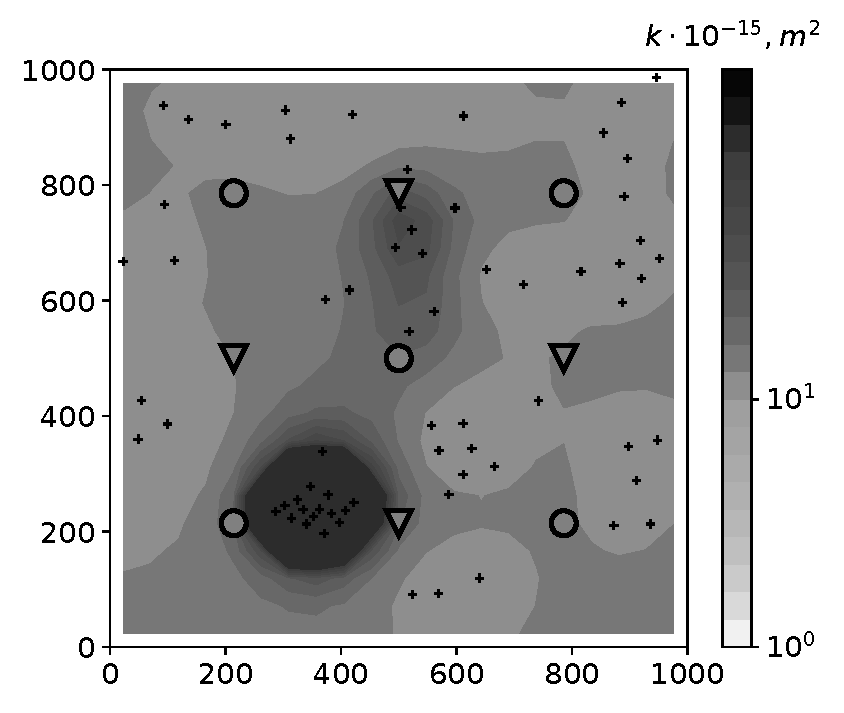
\includegraphics[height=0.80\linewidth]{images/fig5a.eps}\\
		a)
		\label{fig:mob}
	\end{minipage} \hfill
	\begin{minipage}[h]{0.48\linewidth}
		\centering
		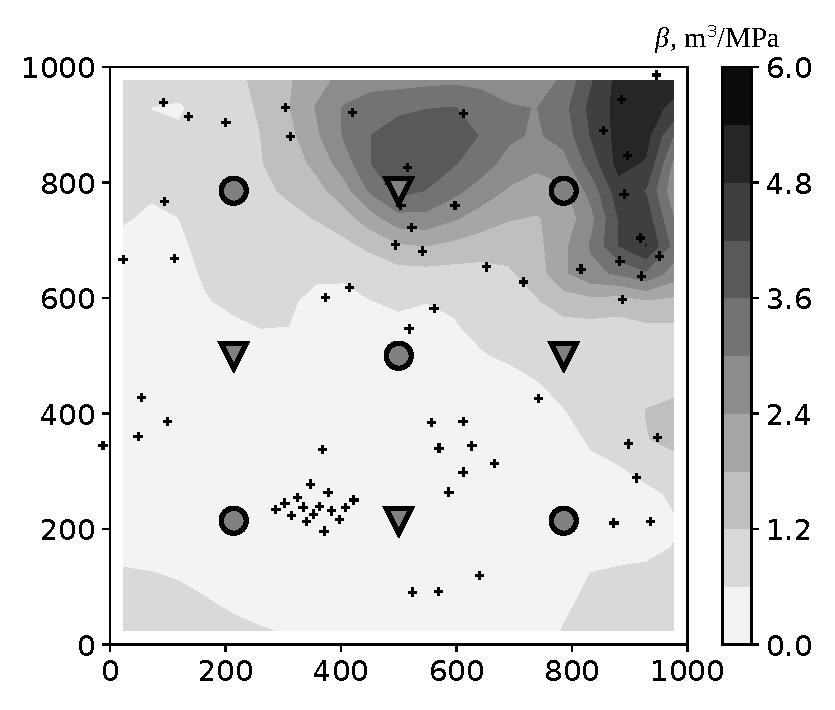
\includegraphics[height=0.80\linewidth]{images/fig5b.eps} \\
		b)
		\label{fig:comp}
	\end{minipage}
	\caption{Восстановленные поля проницаемости (a) и упругоёмкости (b)}
\end{figure}


На рисунках \ref{fig:mob}a и \ref{fig:comp}b чёрными крестиками показаны полученные положения базисов для сети радиально-базисных функций. Можно заметить, что они распределены неравномерно, значительное количество базисов сконцентрировано в области высокопроницаемого включения $k_1$, немного меньше — в области включения $k_2$. Также заметная часть базисов находится в зоне с повышенной упругоёмкостью, хотя и с меньшей концентрацией. В процессе решения алгоритм подбирает положение базисов для наилучшего воспроизведения основных особенностей зональной неоднородности. 

Было проведено количественное сравнение между истинным и восстановленными полями общей подвижности на основе межскважинных связей. Сопоставление значений межскважинных связей представлено в таблице \ref{tabl:connection}. Эти значения были получены путем частичного исключения переменных из численной фильтрационной модели \cite{and}. Высокие значения для соединений I1-P1 и I4-P3 соответствуют зонам (каналам) с высокой проницаемостью. Это подтверждается тем, что порядок ранжирования расчётных значений аналогичен порядку истинных значений. Кроме того, существует удовлетворительный уровень соответствия между значениями коэффициентов взаимовлияния со средней абсолютной погрешностью 6\%. Таким образом, оцененное поле общей подвижности адекватно отражает ключевые особенности исходного поля. 

\begin{table}[h!]
	\caption{Коэффициенты взаимовлияния скважин}	
	\label{tabl:connection}	
	\begin{center}
		\begin{tabular}{c|c|c|c|c}
			\hline
			Well source &  Well drain & True value & Estimated  value & MAPE, \% \\
			\hline
			I1 & P1 & 53.5 & 50.3 & 5.8 \\
			I1 & P3 & 34.1 & 27.4 & 19.7 \\
			I4 & P3 & 33.7 & 34.3 & 1.7 \\
			I2 & P1 & 25.2 & 21.8 & 13.6 \\
			I2 & P3 & 24.2 & 21.6 & 10.7 \\
			I4 & P5 & 21.8 & 20.3 & 7.0 \\
			I3 & P3 & 21.4 & 21.3 & 0.4 \\
			I4 & P4 & 21.0 & 20.3 & 3.4 \\
			I1 & P2 & 20.3 & 20.0 & 1.8 \\
			I2 & P4 & 17.7 & 17.1 & 3.5 \\
			I3 & P2 & 16.9 & 17.0 & 0.4 \\
			I3 & P5 & 16.7 & 17.1 & 2.1 \\
			\hline
		\end{tabular}
	\end{center}
\end{table}

Для реальных нефтяных месторождений величина связей между скважинами обычно достоверно неизвестна. Эти значения могут быть получены с помощью парного гидравлического мониторинга скважин, но подобные исследования проводятся редко. Ввиду этого одним из основных критериев оценки качества адаптации модели является соответствие расчётных и измеренных пластовых давлений. На рис. \ref{fig:cp} приведено сравнение значений фактического и расчетного давлений для скважин. Расчётные значения давления, полученные для модели с восстановленными полями проницаемости и эффективной сжимаемости. На рисунке разными маркерами обозначены значения соответствующих тренировочной (train) и тестовой (test) выборок, соответственно, полыми и заполненными кружками. Удовлетворительное совпадение было получено для тренировочной и тестовой выборок, значения средней относительной погрешности для которых составляют 2,6\% и 3,5\% соответственно. Модель демонстрирует удовлетворительную точность в тестовой выборке, что подтверждает ее прогностические свойства.

\begin{figure}
	\centering
	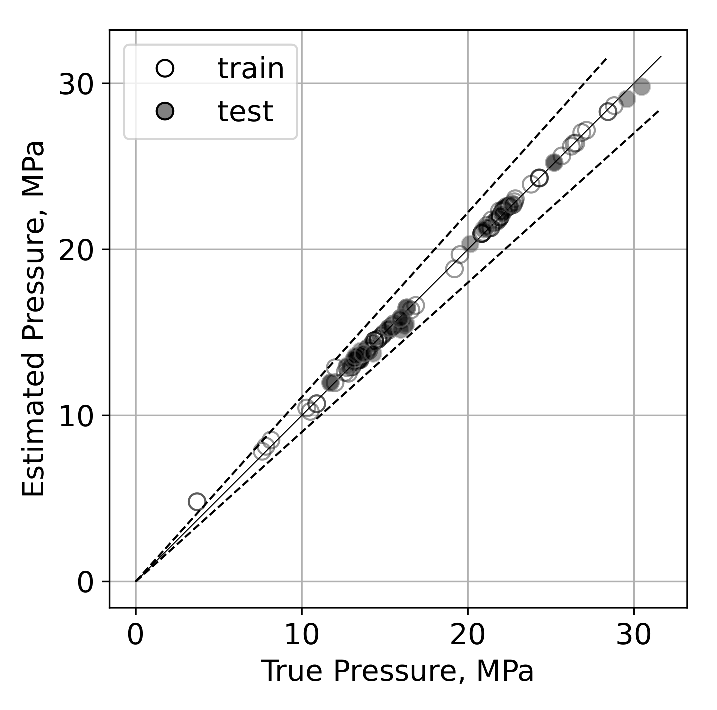
\includegraphics[width=0.5\linewidth]{images/fig6.eps}
	\caption{Сопоставление фактических и расчетных значений пластового давления. Пунктирная линия обозначает интервал отклонения в 10\%}
	\label{fig:cp}
\end{figure}

Количественное сравнение истинных и расчетных значений эффективной сжимаемости показано на рисунке \ref{fig:hist}. На рисунке столбцы 1 и 2 соответствуют истинным и расчетным значениям. Значения были получены путем усреднения значений, полученных с карты, и включены в соответствующий многоугольник Вороного для соответствующей скважины. Как видно на рисунке, алгоритм смог воспроизвести повышенную упругоёмкость в соответствующей зоне (скважины I3, I4 и P5). Несмотря на отличие значений усредненной сжимаемости качественное соответствие фактических и расчетных значений достигнуто.

\begin{figure}
	\centering
	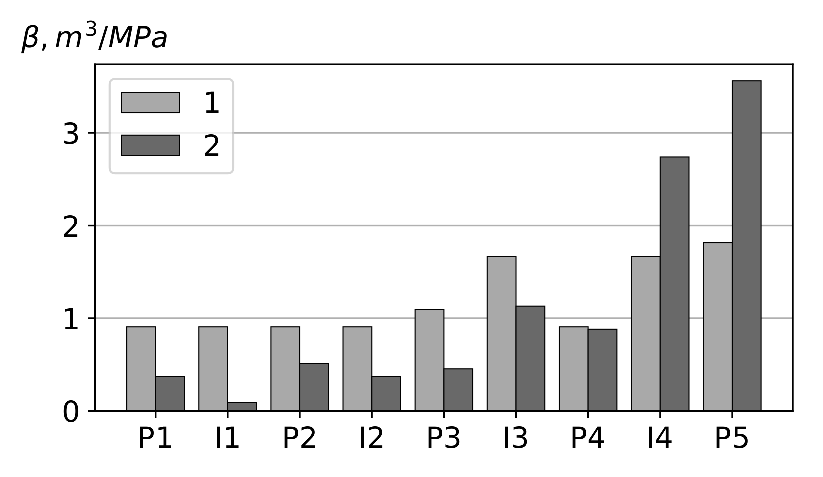
\includegraphics[width=0.7\linewidth]{images/fig7.eps}
	\caption{Сопоставление фактических (1) и восстановленных (2) значений усредненной вблизи скважин упругоёмкости}
	\label{fig:hist}
\end{figure}


\section{CONCLUSIONS}
В статье представлен подход к совместному использованию теории фильтрации с методами машинного обучения для решения задачи адаптации модели на исторические данные. На примере синтетической модели элемента нефтяного месторождения с регионально неоднородными полями проницаемости и упругоёмкости показана реализация данного подхода.

Настройка однофазной фильтрационной модели на исторические данные была достигнута путем восстановления полей проницаемости и упругоемкости при использовании сети радиальных базисных функций и полносвязного линейного слоя. На основе восстановленного поля проницаемости были рассчитаны коэффициенты взаимовлияния скважин, которые количественно удовлетворительно соответствуют истинному значению. На основе восстановленного поля упругоемкости методом усреднения вблизи скважин были рассчитаны средние значения показателей. Эти средние значения также качественно соответствуют исходным. Таким образом, предлагаемый подход позволяет восстановить характерный вид зональной неоднородности в моделируемом объекте.

Решение обратной задачи было получено для случая, когда в исходном наборе данных отсутствовало значительное количество данных. Это делает предлагаемый метод пригодным для практического применения. Данный алгоритм имеет универсальный характер и может быть использован в сочетании с более сложными алгоритмами машинного обучения в будущем.

\section{FUNDING}
«Исследование выполнено за счет гранта Российского научного фонда № 24-21-00468,
 \\ https://rscf.ru/project/24-21-00468/»
 
 \begin{thebibliography}{20}
	
\bibitem{mus1} E. N. Musakaev, S. P. Rodionov and N. G. Musakaev, "Hierarchical Approach to Identifying Fluid Flow Models in a Heterogeneous Porous Medium", Mathematics, 9(24), 3289 (2021).

\bibitem{bek} A. D. Bekman, T. A. Pospelova and D. V. Zelenin,  "A new approach to water cut forecasting based on results of capacitance resistance modeling", Vestn. Tyumen. Univ., Fiz. Mat. Model. Neft’, Gaz, Energet. 6 (1(21)), 192–207 (2020).

\bibitem{pot} K.A. Potashev, R.R. Akhunov and  A.B. Mazo, "Calculation of the flow rate between wells in the flow model of an oil reservoir using streamlines", Georesources. 24(1), 27–35 (2022).

\bibitem{ele} A. V. Elesin, A. Sh. Kadyrova, "Determination of the Anisotropic Reservoir Permeability by Liquid Flow Rate Measurements at Wells under Conditions of Three-Phase Filtration", Lobachevskii J. Math.
{\bf 44}, 1593--1599 (2023).

\bibitem{kos} V. P. Kosyakov, "Investigation of the Influence of Weight Coefficients in Solving the Problem of Permeability Identification for an Oil Field", Lobachevskii J. Math.
{\bf 44}, 1721--1727 (2023).

\bibitem{tem}  P. Temirchev, M. Simonov, R. Kostoev, E. Burnaev, I. Oseledets, A. Akhmetov, A. Margarit, A. Sitnikov and D. Koroteev, "Deep neural networks predicting oil movement in a development unit", Journal of Petroleum Science and Engineering. 184. 106513 (2020).

\bibitem{uma} A. W. Umanovskiy, "Proxy modeling pf reservoir hydrodynamics with graph neural networks",Vestn. Tyumen. Univ., Fiz. Mat. Model. Neft’, Gaz, Energet. 8 (3(31)), 155-177 (2022).

\bibitem{kos2} V. P. Kosyakov and D. Yu. Legostaev, “Using elements of machine learning to solve the inverse problem of reconstructing the hydraulic conductivity feld for a fltration problem,” Vestn. Tyumen. Univ., Fiz. Mat. Model. Neft’, Gaz, Energet. 8 (2 (30)), 129–149 (2022).

\bibitem{bas}
K. S. Basniev, N. M. Dmitriev, R. D. Kanevskaya, and V. M. Maksimov, \textit{Underground Hydromechanics} (Inst. Komp'yut. Issled., Moscow, 2006) [in Russian].

\bibitem{abd}
A. Satter, G. M. Iqbal, \textit{Reservoir Engineering: The Fundamentals, Simulation, and Management of Conventional and Unconventional Recoveries} (Gulf Professional Publishing, 2016).

\bibitem{kos3} V.P.Kosyakov, S.P.Rodionov, "Optimal control of wells on the basis of two-phase filtration equations",  Tr. MFTI. 8(3), 79-90 (2016).

\bibitem{far} P. E. Farrell, D. A. Ham, S. W. Funke and M. E. Rognes, "Automated Derivation of the Adjoint of High-Level Transient Finite Element Programs",SIAM Journal on Scientific Computing, 35(4) 369-393 (2013).

\bibitem{inn}  M. Innes, E. Saba, K. Fischer, D. Gandhi, M. C. Rudilosso, N. M. Joy, T. Karmali, A. Pal and V. B. Shah, "Fashionable Modelling with Flux", ArXiv. 1811.01457 (2018).

\bibitem{and} V. B. Andreev, \textit{Numerical methods}. (М.: MAKS Press)[in Russian].

\bibitem{azi} H. Aziz, E. Settari. \textit{Mathematical modeling of reservoir systems}.  M.-Izhevsk: Institute for Computer Research, 2004. [in Russian]


\end{thebibliography}

\end{document}
